\documentclass[a5paper]{article}
\usepackage[a5paper, top=8mm, bottom=8mm, left=8mm, right=8mm]{geometry}

\usepackage{polyglossia}
\setdefaultlanguage[babelshorthands=true]{russian}

\usepackage{fontspec}
\setmainfont{FreeSerif}
\newfontfamily{\russianfonttt}[Scale=0.7]{DejaVuSansMono}

\usepackage[font=scriptsize]{caption}

\usepackage{amsmath}
\usepackage{amssymb,amsfonts,textcomp}
\usepackage{color}
\usepackage{array}
\usepackage{hhline}
\usepackage{cite}

\usepackage[hang,multiple]{footmisc}
\renewcommand{\footnotelayout}{\raggedright}

\PassOptionsToPackage{hyphens}{url}\usepackage[xetex,linktocpage=true,plainpages=false,pdfpagelabels=false]{hyperref}
\hypersetup{colorlinks=true, linkcolor=blue, citecolor=blue, filecolor=blue, urlcolor=blue, pdftitle=1, pdfauthor=, pdfsubject=, pdfkeywords=}

\usepackage{tabu}

\usepackage{graphicx}
\usepackage{indentfirst}
\usepackage{multirow}
\usepackage{subfig}
\usepackage{footnote}
\usepackage{minted}

\sloppy
\pagestyle{plain}

\title{Необязательная практика 4: Ещё примеры архитектур}

\date{}

\begin{document}

\maketitle
\thispagestyle{empty}

\section{Git}

Имеет смысл посмотреть первоисточники: краткий обзор архитектуры Git в <<The Architecture of Open Source Applications>>\footnote{\url{http://aosabook.org/en/git.html}} и, что полезнее, но длиннее, глава 10 Git Book\footnote{\url{https://git-scm.com/book}}. 

Git, как известно, распределённая система контроля версий, поэтому весь репозиторий вынужден хранить локально и, если мы никуда push-ить не собираемся, как раз представляет собой локальную version control system (VCS), которую надо сделать в этой задаче (пользоваться гитом в решении, естественно, можно только по прямому назначению). Когда мы набираем \mintinline{text}|git init|, создаётся папка \mintinline{text}|.git|, где лежит вся информация гитового репозитория. Она имеет следующую структуру:

\begin{itemize}
	\item \textbf{HEAD} --- ссылка на текущую ветку, которую зачекаутили в рабочей папке;
	\item \textbf{index} --- staging area, то место, где формируется информация о текущем коммите;
	\item \textbf{config} --- конфигурационные опции гита для этого репозитория;
	\item \textbf{description} --- <<is only used by the GitWeb program, so don’t worry about it>> (c) Git Book;
	\item \textbf{hooks/} --- хук-скрипты (возможность исполнить произвольный код при каком-то действии типа коммита), про которые мы сейчас не будем и в домашке их поддерживать не надо;
	\item \textbf{info/} --- тоже локальные настройки репозитория, сюда можно вписать игнорируемые файлы, которые вы не хотите писать в .gitignore, чтобы их не коммитить;
	\item \textbf{objects/} --- самое интересное, тут лежит собственно то, что хранится в репозитории;
	\item \textbf{refs/} --- тут лежат указатели на объекты из objects (ветки, как мы увидим в дальнейшем);
	\item \textbf{...} --- прочие штуки, которые появляются в процессе жизни репозитория и нам пока не интересны.
\end{itemize}

Гит вообще появился как набор утилит, которые позволяют быстро сделать систему контроля версий, а не как полноценная система контроля версий, так что у гита, помимо общеизвестных команд, есть и команды, позволяющие напрямую работать с репозиторием и делать с ним вручную ужасные вещи. Сам по себе репозиторий в гите --- это просто хеш-таблица, которая отображает SHA-1-хеш файла в содержимое файла, ничего более. Можно класть в неё объекты (даже не обязательно файлы), можно получать. Например, вот так:
\begin{minted}{bash}
$ git init test
Initialized empty Git repository in /tmp/test/.git/
$ cd test
$ find .git/objects
.git/objects
.git/objects/info
.git/objects/pack

$ echo 'test content' | git hash-object -w --stdin
d670460b4b4aece5915caf5c68d12f560a9fe3e4

$ find .git/objects -type f
.git/objects/d6/70460b4b4aece5915caf5c68d12f560a9fe3e4
\end{minted}

Создали пустой репозиторий, гит нам создал структуру папок \mintinline{bash}|.git/objects|, пока пустую. Командой \mintinline{text}|git hash-object| мы положили в репозиторий новый объект --- строчку \mintinline{bash}|'test content'|. Ключ \mintinline{bash}|-w| означает, что надо не просто посчитать хеш объекта, но и реально записать его на диск, ключ \mintinline{bash}|--stdin| означает, что содержимое объекта надо получить из входного потока, а не из файла. Вызов этой команды вернул нам SHA-1-хеш того, что получилось, и заодно создал файл на диске с содержимым, положив его в \mintinline{bash}|.git/objects|, в подпапку, называющуюся как первые два символа хеша, и в файл, называющийся как остальные 38 символов хеша.

Как достать то, что мы сохранили, обратно:
\begin{minted}{text}
$ git cat-file -p d670460b4b4aece5915caf5c68d12f560a9fe3e4
test content
\end{minted}

Команда \mintinline{bash}|git cat-file| показывает содержимое файла, ключ \mintinline{bash}|-p| говорит определить тип объекта и красиво показать его содержимое.

Уже можно сделать версионный контроль вручную с использованием рассмотренных команд (правда, для этого нам потребуется настоящий файл, версионировать строку, как в предыдущем примере, не интересно):

\begin{minted}{bash}
$ echo 'version 1' > test.txt
$ git hash-object -w test.txt
83baae61804e65cc73a7201a7252750c76066a30

$ echo 'version 2' > test.txt
$ git hash-object -w test.txt
1f7a7a472abf3dd9643fd615f6da379c4acb3e3a

$ find .git/objects -type f
.git/objects/1f/7a7a472abf3dd9643fd615f6da379c4acb3e3a
.git/objects/83/baae61804e65cc73a7201a7252750c76066a30
.git/objects/d6/70460b4b4aece5915caf5c68d12f560a9fe3e4

$ git cat-file -p 83baae61804e65cc73a7201a7252750c76066a30 > test.txt
$ cat test.txt
version 1

$ git cat-file -p 1f7a7a472abf3dd9643fd615f6da379c4acb3e3a > test.txt
$ cat test.txt
version 2
\end{minted}

Каждая новая версия в данном случае хранится как отдельный объект, но всему своё время.

Объект, кстати, называется <<blob>> (Binary Large OBject), и он хранит только данные, так что даже имя файла в нём не хранится, а, наверное, хотелось бы. За хранение имени файла, а также за хранение папок и вообще иерархии объектов отвечает объект <<tree>>. Например, вот так могло бы выглядеть дерево, на которое указывает коммит \mintinline{text}|master| в некотором репозитории (два файла и одно поддерево):

\begin{minted}{text}
$ git cat-file -p master^{tree}
100644 blob a906cb2a4a904a152e80877d4088654daad0c859      README
100644 blob 8f94139338f9404f26296befa88755fc2598c289      Rakefile
040000 tree 99f1a6d12cb4b6f19c8655fca46c3ecf317074e0      lib
\end{minted}

Синтаксис \mintinline{text}|master^{tree}| говорит, что надо отобразить master как tree-объект, а не как commit-объект. Вот так можно себе представить дерево, приведённое в примере:

\begin{center}
	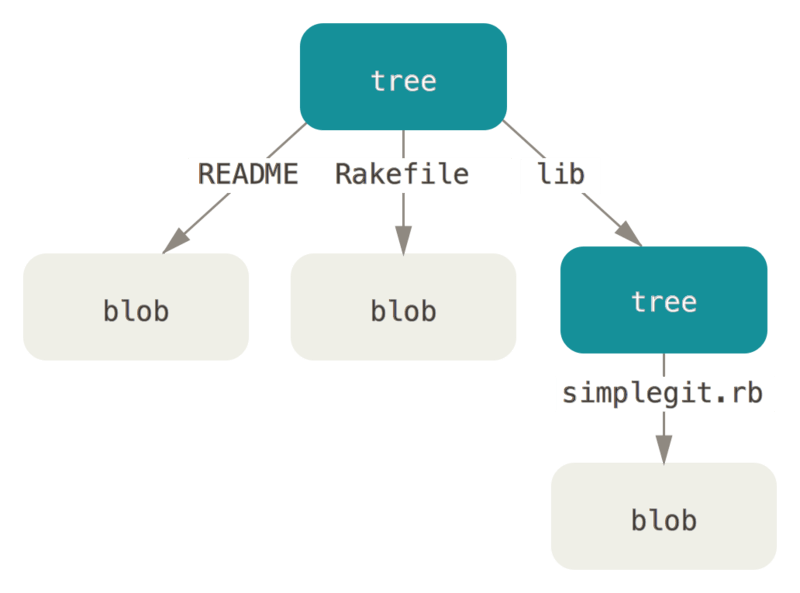
\includegraphics[width=0.5\textwidth]{gitTreeObject.png}
\end{center}

Вот примерная UML-диаграмма классов всех объектов, которые могут находиться в гитовом репозитории:
\begin{center}
	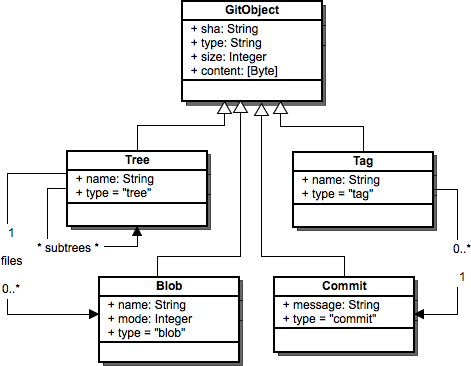
\includegraphics[width=0.7\textwidth]{gitDataStructure.png}
\end{center}

Все они являются объектами, поэтому имеют свой SHA-1-хеш, тип, который позволяет их отличить друг от друга, размер и данные. Blob и Tree мы уже видели, Tree содержит в себе поддеревья и Blob-ы. Осталось разобраться с коммитами и тэгами. 

Коммиты нужны для хранения метаинформации --- кто сделал изменение, когда и почему. Дерево ничего такого не хранит, в этом смысле оно напоминает узел файловой системы (в UNIX-подобных системах распространён термин inode), так что на объекты из дерева ссылаются коммит-объекты. Вот так это выглядит:
\begin{minted}{text}
$ echo 'first commit' | git commit-tree d8329f
fdf4fc3344e67ab068f836878b6c4951e3b15f3d

$ git cat-file -p fdf4fc3
tree d8329fc1cc938780ffdd9f94e0d364e0ea74f579
author Scott Chacon <schacon@gmail.com> 1243040974 -0700
committer Scott Chacon <schacon@gmail.com> 1243040974 -0700

first commit
\end{minted}

Ещё, что не показано на картинке, но тоже есть --- коммит хранит список коммитов-родителей, но вообще понятие <<родитель>> для коммита связано с ветками, поэтому про них чуть попозже. Вот, наверное, знакомая картинка про то, как коммиты можно представлять себе в виде указателей на узлы дерева в базе:

\begin{center}
	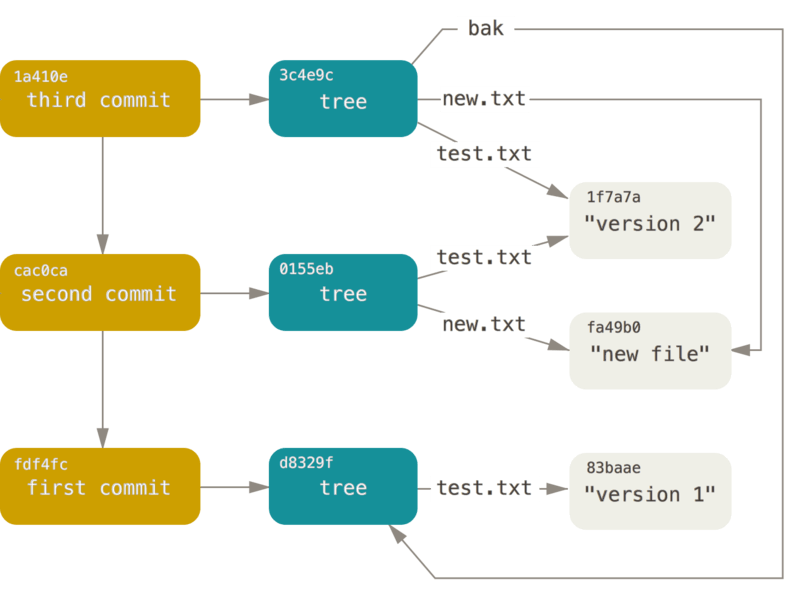
\includegraphics[width=0.7\textwidth]{gitCommitObjects.png}
\end{center}

Теперь у нас есть объекты, хранящие в себе содержимое файлов (blob-ы), объекты, хранящие в себе структуру файлов и их имена (tree-объекты), объекты, хранящие в себе информацию об истории модификаций первых двух видов объектов, и уже, в принципе, система контроля версий могла бы получиться. Но пользоваться ей было бы очень неудобно, потому что каждый объект идентифицируется только своим SHA-1-хешем, и чтобы делать что-нибудь содержательное, надо было бы эти хеши помнить. Чтобы с этим помочь, придуманы references. Reference --- это просто ссылка на коммит. Reference даже не объект, это просто файл, внутри которого лежит SHA-1-хеш объекта из базы. При этом reference-ы бывают двух типов --- head-ы и tag-и. Они хранятся в папке \mintinline{text}|.git/refs|, \mintinline{text}|.git/refs/heads| и \mintinline{text}|.git/refs/tags| соответственно. Мы можем сделать свою собственную ветку, создав сами такой файл:

\begin{minted}{text}
$ echo "1a410efbd13591db07496601ebc7a059dd55cfe9" > .git/refs/heads/master

$ git log --pretty=oneline master
1a410efbd13591db07496601ebc7a059dd55cfe9 third commit
cac0cab538b970a37ea1e769cbbde608743bc96d second commit
fdf4fc3344e67ab068f836878b6c4951e3b15f3d first commit
\end{minted}

Совсем вручную это делать можно, но не принято, есть команда \verb|git update-ref|, которая, во-первых, проверяет, что ref создаётся в правильной папке, во-вторых, заносит действие с reference в так называемый reflog, про который тоже чуть попозже, но вообще --- это штука, которая помнит, что происходило со ссылками и может помочь востановить случайно удалённую ветку. Традиционная картинка, поясняющая суть ссылок:

\begin{center}
	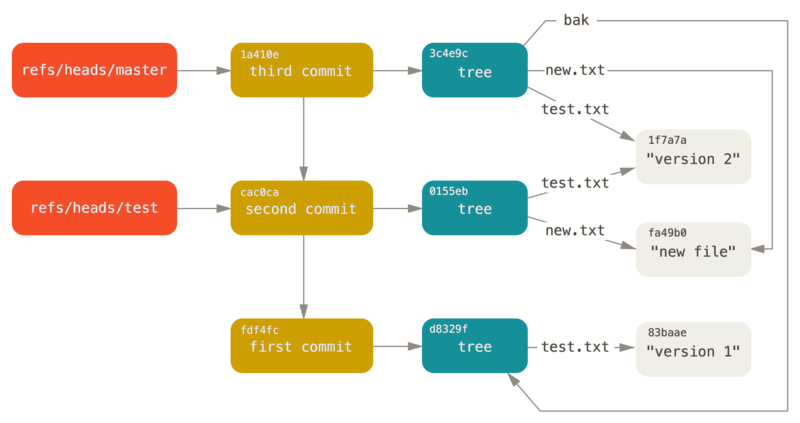
\includegraphics[width=0.9\textwidth]{gitRefs.png}
\end{center}

Среди всех ссылок выделяется самая главная, та, которая соответствует ветке, лежащей сейчас в рабочей копии. Она внезапно хранится не в \mintinline{text}|.git/refs|, а прямо в корне папки \mintinline{text}|.git|, в файле, который называется \mintinline{text}|HEAD|. Причём это даже не ссылка, а символическая ссылка, то есть ссылка на ссылку:

\begin{minted}{text}
$ cat .git/HEAD
ref: refs/heads/master

$ git symbolic-ref HEAD refs/heads/test
$ cat .git/HEAD
ref: refs/heads/test
\end{minted}

Команда \mintinline{text}|git symbolic-ref| нужна для <<вежливого>> обновления символической ссылки, которая проверяет корректность того, что происходит. Таким нехитрым образом можно переключаться между ветками, но обратите внимание, что \mintinline{text}|index| ничего про это не знает, так что файлы из старой ветки будут считаться добавленными к коммиту, потому что они были в её индексе и никто их оттуда не убрал. Так что \mintinline{text}|git checkout| всё-таки не только обновляет HEAD.

Последний из объектов, который надо рассмотреть --- это тэги. Тэг --- это просто указатель на коммит. Ну, на самом деле, не всё так просто, потому что мы видели его на диаграмме с объектами в базе, а reference --- не объект. Дело в том, что тэги бывают двух типов --- легковесные и аннотированные. Легковесный тэг --- это просто ссылка на коммит, которая никогда никем не двигается (её можно продвинуть вручную, но это плохо, поскольку тогда у людей, имеющих копии вашего репозитория, тэги могут начать не совпадать). Аннотированный тэг --- это уже полноценный объект, который указывает на коммит, и нужен он для того, чтобы иметь возможность добавить к тэгу разную метаинформацию типа автора, сообщения и даты.

Пример, как сделать вручную легковесный тэг:
\begin{minted}{text}
git update-ref refs/tags/v1.0 cac0cab538b970a37ea1e769cbbde608743bc96d
\end{minted}

А вот аннотированный тэг и как он хранится:
\begin{minted}{text}
$ git tag -a v1.1 1a410efbd13591db07496601ebc7a059dd55cfe9 -m 'test tag'

$ git cat-file -p 9585191f37f7b0fb9444f35a9bf50de191beadc2
object 1a410efbd13591db07496601ebc7a059dd55cfe9
type commit
tag v1.1
tagger Scott Chacon <schacon@gmail.com> Sat May 23 16:48:58 2009 -0700

test tag
\end{minted}

Казалось бы, теперь всё, но тут мы вспоминаем, что все объекты в репозитории всё ещё хранятся целиком, так что если у нас есть длиннющий исходник и мы в нём поменяли одну строчку, у нас получится два длиннющих исходника. Самое удивительное, что, в общем-то, в гите поначалу так и есть, репозиторий некоторое время просто раскопирует изменённые файлы. Естественно, файлы сжимаются zlib-ом, так что занимают чуть меньше места, чем могли бы, но всё равно, для системы контроля версий такая ситуация довольно странна. На помощь приходят pack-файлы:

\begin{minted}{text}
$ git gc
Counting objects: 18, done.
Delta compression using up to 8 threads.
Compressing objects: 100% (14/14), done.
Writing objects: 100% (18/18), done.
Total 18 (delta 3), reused 0 (delta 0)

$ find .git/objects -type f
.git/objects/bd/9dbf5aae1a3862dd1526723246b20206e5fc37
.git/objects/d6/70460b4b4aece5915caf5c68d12f560a9fe3e4
.git/objects/info/packs
.git/objects/pack/pack-978e03944f5c581011e6998cd0e9e30000905586.idx
.git/objects/pack/pack-978e03944f5c581011e6998cd0e9e30000905586.pack
\end{minted}

Тут мы выполнили команду \mintinline{text}|git gc| (Garbage Collect), в результате которой некоторые <<нормальные>> объекты удалились (на самом деле, все кроме <<висячих>>, то есть недостижимых по ссылкам) и появилось два файла: \mintinline{text}|.idx| и \mintinline{text}|.pack|. Второй файл содерхит упакованными все наши объекты, и тут уже применяется дельта-компрессия, причём, что интересно, последняя версия файла хранится целиком, а предыдущие версии --- как дельты относительно более свежей версии, то есть как бы <<назад>> (что логично, скорее всего, последняя версия нужна чаще). Первый файл --- это оглавление для второго файла, именно его передают по сети, когда делается git push/git pull и локальный или удалённый гит пытается понять, какой информации у него нету. Вот так примерно это выглядит:

\begin{center}
	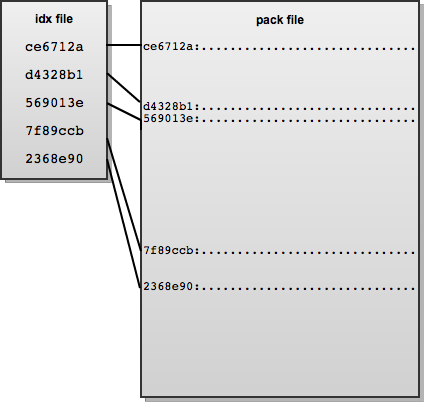
\includegraphics[width=0.6\textwidth]{gitPackFiles.png}
\end{center}

Упаковка объектов в .pack-файлы происходит, когда:
\begin{itemize}
	\item Выполняется git push;
	\item Слишком много <<свободных>> объектов (порядка 7000);
	\item Вручную вызвана git gc.
\end{itemize}

Если pack-файл уже есть, то новые объекты могут упаковаться в новый файл, оставив старый неизменённым, а может произойти перепаковка и несколько .pack-файлов будут слиты в один (важно понимать, что .pack-файлов может быть несколько и вся работа с ними скрыта от пользователя системы контроля версий). Почему всё так хитро --- упаковка в .pack-файл требует пересчёта дельт и вообще очень трудоёмкая операция, так что делать её каждый коммит было бы очень раздражающе для пользователя. Есть ещё команда \mintinline{text}|git gc --auto|, которая проверяет, не надо ли запаковать объекты, она вызывается при каждом коммите и, как правило, ничего не делает, иногда всё-таки вызывая \mintinline{text}|git gc|. Внутрь pack-файла можно посмотреть командой \mintinline{text}|git verify-pack|, не то чтобы сильно полезно на практике, так что подробности в Git Book.

Теперь бонусный контент про то, как устроен reflog и как восстановить случайно удалённую ветку. Все нормальные команды гита записывают всё, что оин делали с reference-ами в файлы в папке \mintinline{text}|logs|, где, в частности, лежит лог того, что происходило со ссылкой \mintinline{text}|HEAD|, и его можно просмотреть командой \mintinline{text}|git reflog|:

\begin{minted}{text}
$ git reflog
1a410ef HEAD@{0}: reset: moving to 1a410ef
ab1afef HEAD@{1}: commit: modified repo.rb a bit
484a592 HEAD@{2}: commit: added repo.rb
\end{minted}

Или получить более подробную информацию командой \mintinline{text}|git log -g|:

\begin{minted}{text}
$ git log -g
commit 1a410efbd13591db07496601ebc7a059dd55cfe9
Reflog: HEAD@{0} (Scott Chacon <schacon@gmail.com>)
Reflog message: updating HEAD
Author: Scott Chacon <schacon@gmail.com>
Date:   Fri May 22 18:22:37 2009 -0700

    third commit
$ git branch recover-branch ab1afef
\end{minted}

А теперь как более капитально прострелить себе ногу. Шаг 1, удаляем ветку:

\begin{minted}{text}
$ git branch -D master
\end{minted}

Шаг второй, сносим все логи, чтобы нельзя было восстановить ветку по SHA-1-хешу последнего коммита, на который она указывала:

\begin{minted}{text}
$ rm -Rf .git/logs/
\end{minted}

Казалось бы, всё, репозиторий запорот и надо делать домашку заново? Нет, если база объектов на месте, можно воспользоваться командой \mintinline{text}|git fsck --full|, которая распечатает нам все висячие объекты вместе с их хешами:

\begin{minted}{text}
$ git fsck --full
Checking object directories: 100% (256/256), done.
Checking objects: 100% (18/18), done.
dangling blob d670460b4b4aece5915caf5c68d12f560a9fe3e4
dangling commit ab1afef80fac8e34258ff41fc1b867c702daa24b
dangling tree aea790b9a58f6cf6f2804eeac9f0abbe9631e4c9
dangling blob 7108f7ecb345ee9d0084193f147cdad4d2998293
\end{minted}

Теперь мы можем посмотреть на них командой \mintinline{text}|git cat-file -p|, выбрать тот, который больше всего похож на последний коммит той ветки, которую мы удалили, и восстановить ветку по его хешу: \mintinline{text}|git branch recover-branch ab1afef|. Ещё позитивно то, что Git не удалит даже <<висячие>> объекты несколько месяцев, если его явно не попросить, несмотря на то, как расшифровывается имя команды \mintinline{text}|git gc|, так что если вы потеряли ветку, то с большой вероятностью она всё ещё где-то есть и её можно восстановить.

\end{document}
